%!TEX root = ../template.tex
%%%%%%%%%%%%%%%%%%%%%%%%%%%%%%%%%%%%%%%%%%%%%%%%%%%%%%%%%%%%%%%%%%%%
%% chapter5.tex
%% NOVA thesis document file
%%
%% Chapter with lots of dummy text
%%%%%%%%%%%%%%%%%%%%%%%%%%%%%%%%%%%%%%%%%%%%%%%%%%%%%%%%%%%%%%%%%%%%

\typeout{NT FILE chapter7.tex}%

\chapter{OCamlFLAT / OFLAT}
\label{cha:current_system}

This chapter presents the OCamlFLAT/OFLAT system as it stands currently. The system
is built of two parts, the web application, which offers a graphical interface to
the system, and the library it is built upon, which contains the logical part
of the system. By understanding the OCamlFLAT/OFLAT system's design and limitations,
we can then have a better understanding of the new functionalities to be added.

\section{OCamlFLAT Library}
The OCamlFLAT library is structured to provide a clear and modular framework for working with formal languages and automata. 
Its hierarchical module design starts with abstract concepts at the top, simplifying code organization and future expansions.
At the top is the \textbf{Entity} module, which generalizes all other modules. 
The \textbf{Exercise} module supports exercise creation and validation, while the \textbf{Model} module offers shared utilities for all FLAT models, 
encouraging consistent implementations and code reuse.
In this thesis, support for finite state transducers will be added to the library as well as all its necessary operations, which will be implemented as a new module.

Supporting modules handle essential tasks such as JSON serialization, error management, and foundational type definitions. 
Among these, the \textbf{BasicTypes} module plays a key role by defining core constructs like symbols, words, states, 
and transitions—elements central to modeling automata and formal languages.

Each formal model in the library is represented by a pair of modules: one for auxiliary tasks like parsing and formatting, and another dedicated to core logic. The main logic modules include:
\begin{itemize}
\item \textbf{Regular Expression Module}: Implements word generation, word acceptance checking, conversion of regular expressions into finite automata, and simplification routines.
\item \textbf{Finite Automaton Module}: Provides functions for creating, editing, minimizing, and analyzing finite automata, including conversions between deterministic and nondeterministic forms and detection of useful states.
\item \textbf{Context Free Grammar Module}: Offers support for word generation and acceptance, validation, removal of left recursion and epsilon productions, and transformations to LL(1) grammars. It also provides computation of First and Follow sets, parsing table construction, and support for LR(0), SLR(1), LR(1), and LALR(1) parsing techniques.
\item \textbf{Pushdown Automaton Module}: Extends FA functionalities to pushdown automata, covering acceptance, generation, and minimization, with mechanisms for validating determinism and identifying productive and reachable states.
\item \textbf{Turing Machine Module}: Handles creation, modification, and analysis of Turing machines, including validation, determinism checking, linear boundedness checking, and conversions to finite automata where appropriate.
\item \textbf{Composition Module}: Supports operations on model compositions, such as union, concatenation, intersection, and Kleene closure.
\item \textbf{Poly Module}: Facilitates type conversions and interactions between different model types, including conversions across regular expressions, finite automata, context-free grammars, PDAs, and TMs.
\item \textbf{Exercises Module}: Manages definition and manipulation of exercises, aligning with the system's pedagogical goals.
\end{itemize}

\section{OFLAT}

OFLAT is a web-based application providing an interactive interface built upon the OCamlFLAT library, 
with an emphasis on ease of use and educational effectiveness. Its design allows users to intuitively create, manipulate, and analyze a wide variety of formal language models.

\subsection{User Interface Layout}

OFLAT's interface is split into two primary sections:
\begin{enumerate}
\item \textbf{Side Menu}: Located on the left (shown in Figure~\ref{fig:oflat_side_menu}), 
this menu lets users choose models such as finite automata, regular expressions, context-free grammars, pushdown automata, and Turing machines. 
It also offers predefined examples for quick loading, options for word operations (acceptance, generation, tracing, conversions), and the ability to import or export models.
\item \textbf{Dynamic Workspace}: On the right side (shown in Figure~\ref{fig:oflat_workspace}), this area dynamically updates based on user interactions. 
It displays the current model visually and provides tools for editing, such as adding or removing states, transitions, or modifying grammar rules. 
The workspace often splits into a left panel for model structure and operations, and a right panel for operation results.
\end{enumerate}

\begin{figure}[htbp]
    \centering
    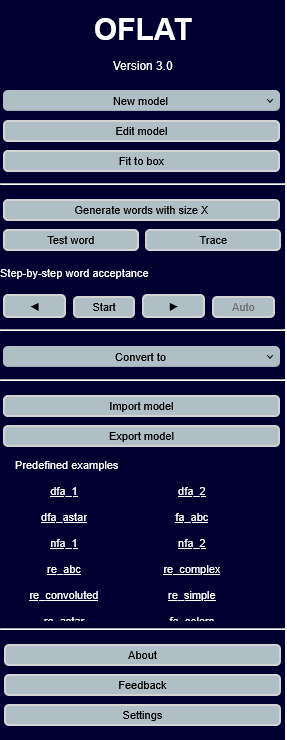
\includegraphics[scale=0.6]{oflat_side_menu.png}
    \caption{OFLAT Side Menu}
    \label{fig:oflat_side_menu}
\end{figure}

\begin{figure}[htbp]
    \centering
    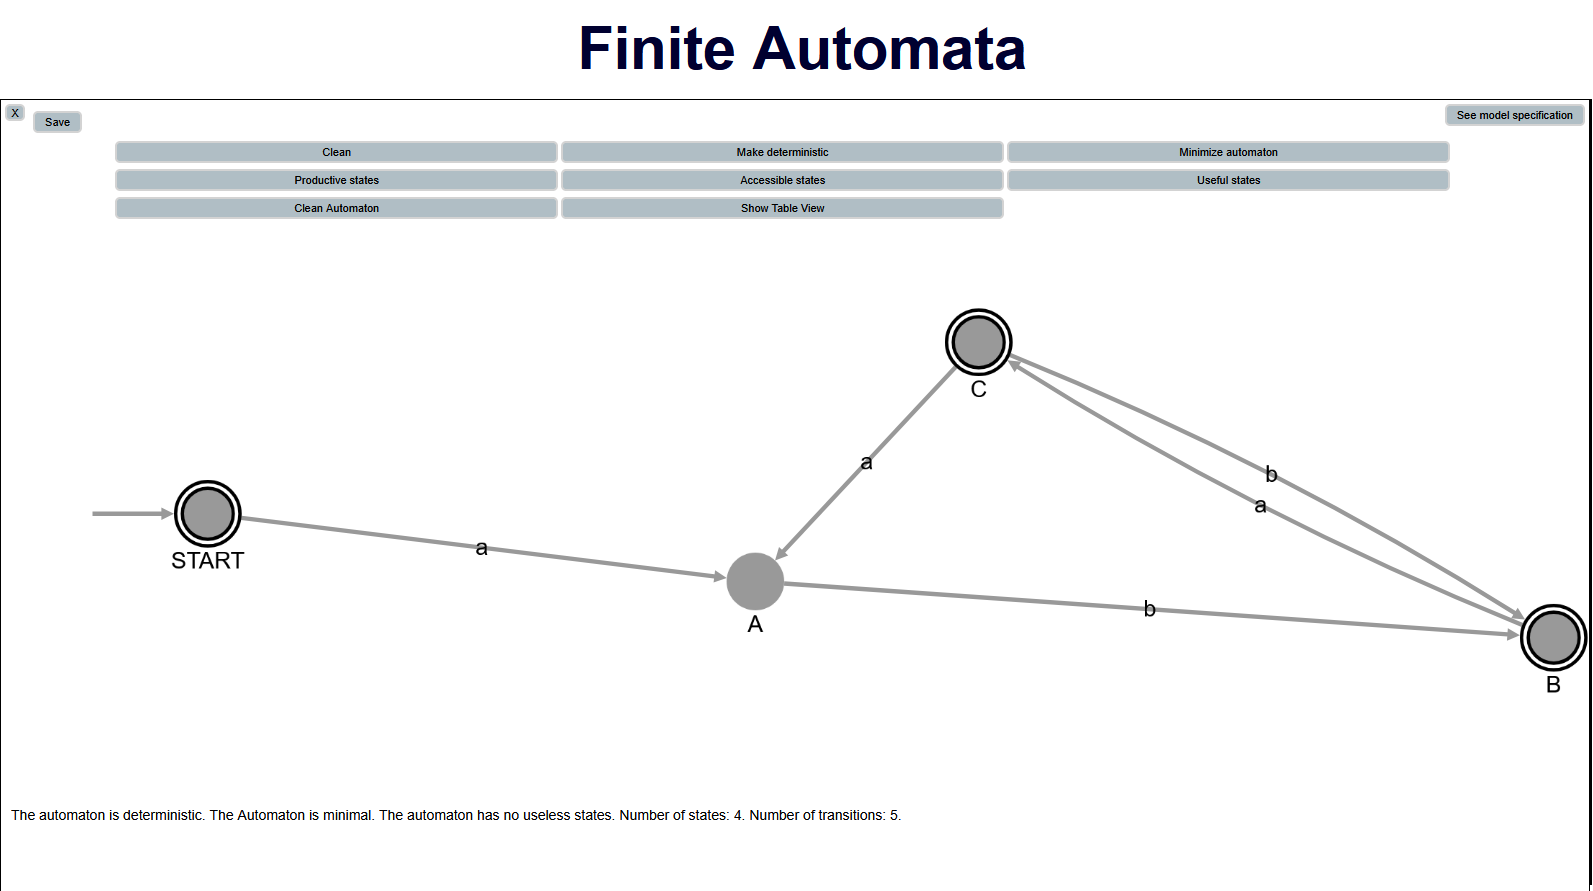
\includegraphics[scale=0.35]{oflat_workspace.png}
    \caption{OFLAT Workspace showing a finite automaton}
    \label{fig:oflat_workspace}
\end{figure}

\subsection{OFLAT Architecture}

The OFLAT web application follows the Model-View-Controller (MVC) design pattern, 
which ensures a clear separation of responsibilities among its components:

\begin{itemize}
    \item \textbf{Model}: The \texttt{OCamlFLAT} library acts as the model layer, 
    handling all the logic and data structures related to formal language theory.
    \item \textbf{View}: This layer includes the graphical components of the system.
    The view modules are responsible for the visual representation of models and for handling user interaction.
    \item \textbf{Controller}: The controller modules process user input and turn them into commands for the view and model.
\end{itemize}
A standard operation in OFLAT typically follows this sequence:
\begin{enumerate}
    \item The user interacts with the interface by providing input.
    \item The controller receives the user command and, using the model (i.e., the OCamlFLAT library), performs the required computations.
    \item The controller then updates the view to display the results.
\end{enumerate}

This modular design enhances the system's maintainability and makes it easier to extend with new features or support for additional formal models in the future.

\section{Conclusion}

Together, the OCamlFLAT library and the OFLAT web interface, provide a platform for learning and exploring formal language concepts through interactive, evolving tools. 
While the system has already achieved significant functionality, further enhancements are necessary to meet its full potential. 
For instance, the absence of a help section and the sometimes overwhelming arrangement of buttons in the interface can hinder user experience.
Nevertheless, OFLAT supports future growth, allowing new models and functionalities to be added.

% \lipsum[1-700]
% \lipsum[1-700]
% \lipsum[1-700]
% \lipsum[1-700]
% \lipsum[1-700]
% \lipsum[1-700]
% \lipsum[1-700]
